% !Mode:: "TeX:UTF-8" 



\BiSection{2.20}{Figures}

\fancyhead[R]{本题2.20由学物理的小李完成}

		\begin{figure}[H] %H为当前位置,!htb为忽略美学标准,htbp为浮动图形
	\begin{minipage}{\linewidth}
		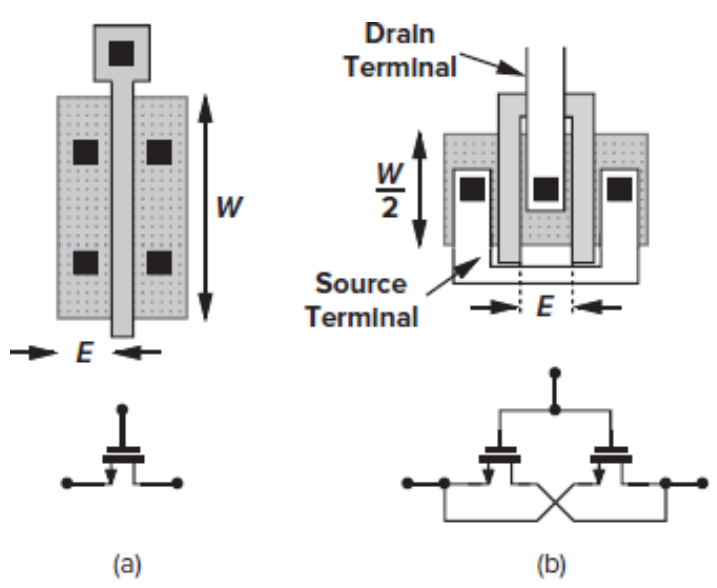
\includegraphics[width=1\linewidth]{2.33-s}
	\end{minipage}
	\caption*{图2.33} %最终文档中希望显示的图片标题
\end{figure}

解:

\scalebox{3}{(1)}

忽略图2.52的边缘,图像看起来一定像四个MOSFETs并联,修改后的图见图1

		\begin{figure}[H] %H为当前位置,!htb为忽略美学标准,htbp为浮动图形
	\begin{minipage}{\linewidth}
		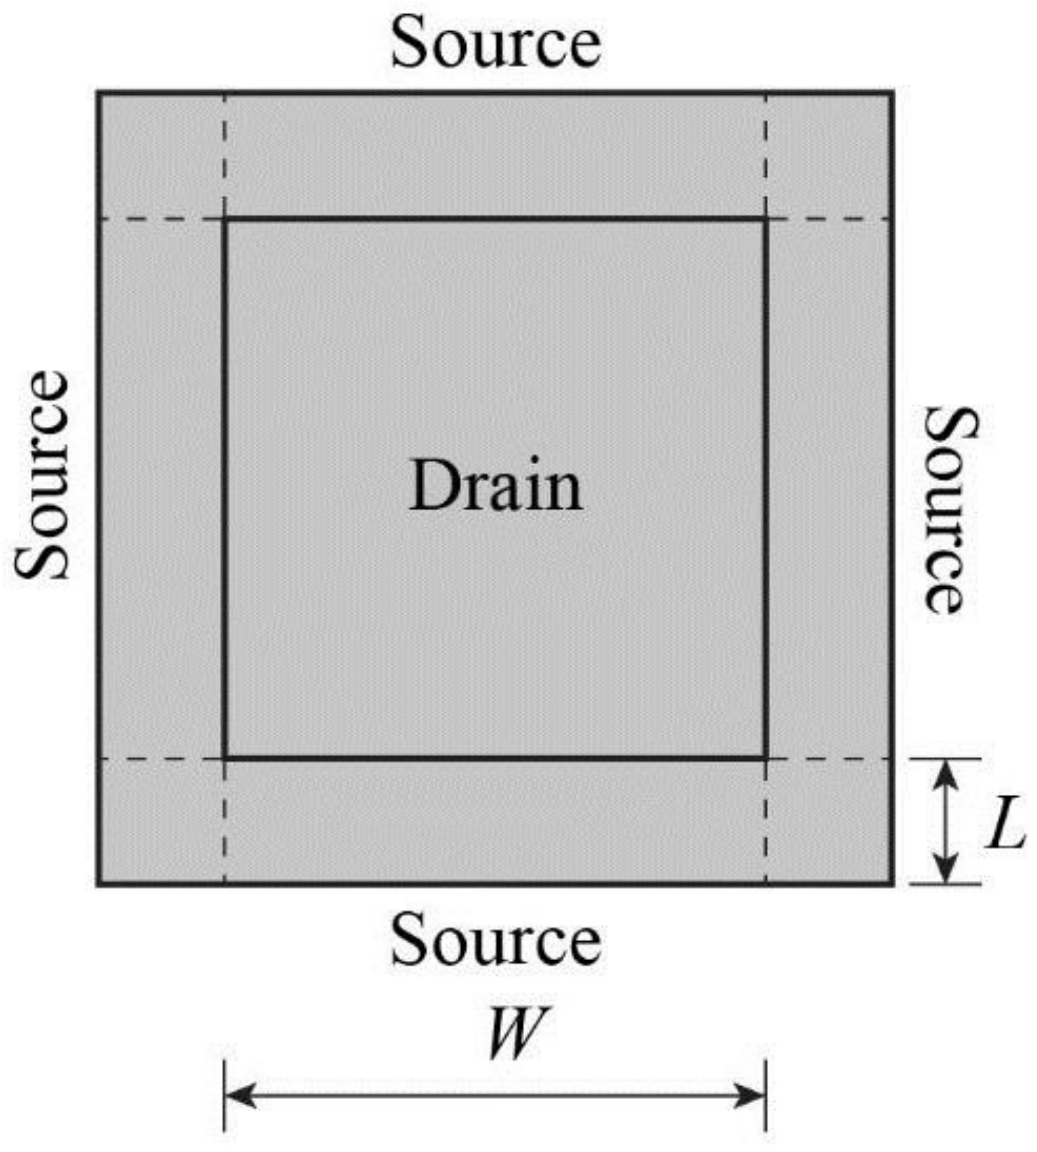
\includegraphics[width=1\linewidth]{2.20-1}
	\end{minipage}
	\caption*{图1} %最终文档中希望显示的图片标题
\end{figure}

“环形”MOS结构工作一定像传统MOSFET,通过改变沟道宽度影响源和漏之间的电子或空穴流动,而沟道宽度被源和漏之间的栅电压控制。

由图1,每个MOSFET宽长比是$\frac{W}{L}$,全部四个MOSFET等效宽长比是$\frac{4W}{L}$

\scalebox{3}{(2)}

由图1,漏结电容$C_{DB}=W^2C_j+4WC_{jsw}$\ding{172}

由图2.33a,漏结电容$C_{DB}=WEC_j+2(W+E)C_{jsw}$,宽乘4则$C_{DB}=4WEC_j+2(4W+E)C_{jsw}=4WEC_j+(8W+2E)C_{jsw}$\ding{173}

由图2.33b,漏结电容$C_{DB}=\frac{W}{2}EC_j+2(\frac{W}{2}+E)C_{jsw}$,宽乘4则$C_{DB}=2WEC_j+(4W+2E)C_{jsw}$\ding{174}

由\ding{172}\ding{173}\ding{174},“环形”结构$C_{jsw}$比折叠和传统结构小,“环形”结构$C_j$比折叠和传统结构大(因为$W>4E$)




